\chapter{La ecuación de Schrödinger en tres dimensiones}\label{ch:b3:schrodinger-three-dimensions}

La pantalla de un televisor moderno brilla con cristales tan pequeños que su
\emph{tamaño} fija su color: un grano de seleniuro de cadmio de cuatro
nanómetros brilla en rojo, y la misma sustancia a dos nanómetros brilla en
azul verdoso. Nada difiere en la química --- solo el tamaño de la caja que
confina a los electrones. El volumen del Año 2 terminó con la mecánica
cuántica en una dimensión: funciones de onda sobre una recta, pozos,
barreras y efecto túnel. Pero los electrones viven en tres dimensiones, y el
paso de la recta al espacio trae física genuinamente nueva: la probabilidad
fluye como una corriente por el espacio, las energías de una caja se
acumulan con \emph{degeneraciones} que delatan su simetría, hay que
\emph{contar} los estados --- el recuento que más adelante gobernará toda la
física estadística --- y los problemas esféricos se reducen, en el caso más
simple, a una ecuación unidimensional disfrazada sobre el radio. Este
capítulo da esos pasos, y sus piezas centrales son el punto cuántico de un
televisor y el núcleo más ligero de la naturaleza.

\section{Funciones de onda en el espacio}

\begin{definition}[Función de onda y probabilidad en tres dimensiones]\label{def:b3:schrodinger-three-dimensions:psi3d}
\index{función de onda!tridimensional}
El estado de una partícula es un campo complejo $\psi(\vect r, t)$ con la
regla de Born
\[
\dd\mathcal P = |\psi(\vect r, t)|^2\,\dd^3r , \qquad
\int|\psi|^2\,\dd^3r = 1 ,
\]
y su evolución es la ecuación de Schrödinger con el laplaciano en lugar de
la derivada segunda:
\[
\iu\hbar\,\frac{\partial\psi}{\partial t}
 = -\frac{\hbar^2}{2m}\,\Delta\psi + V(\vect r)\,\psi ,
\qquad
\Delta = \frac{\partial^2}{\partial x^2} +
\frac{\partial^2}{\partial y^2} + \frac{\partial^2}{\partial z^2} .
\]
Todo lo que estableció el volumen del Año 2 sobrevive literalmente:
linealidad y superposición, estados estacionarios
$\varphi(\vect r)\,\eu^{-\iu Et/\hbar}$ con
$-\tfrac{\hbar^2}{2m}\Delta\varphi + V\varphi = E\varphi$, y el operador
momento, ahora el gradiente $\hat{\vect p} =
-\iu\hbar\vect\nabla$.
\end{definition}

\begin{proposition}[La probabilidad fluye: la corriente]\label{prop:b3:schrodinger-three-dimensions:current}
\index{corriente de probabilidad}
La densidad $\rho = |\psi|^2$ obedece a una ecuación de continuidad,
\[
\frac{\partial\rho}{\partial t} + \operatorname{div}\vect\jmath = 0 ,
\qquad
\vect\jmath = \frac{\hbar}{m}\,
\operatorname{Im}\big(\psi^*\vect\nabla\psi\big) :
\]
la probabilidad se conserva localmente, transportada por la corriente
$\vect\jmath$ --- para una onda plana $A\eu^{\iu\vect k\cdot\vect r}$,
$\vect\jmath = |A|^2\hbar\vect k/m = \rho\vect v$, un flujo uniforme;
para cualquier $\varphi$ real, $\vect\jmath = \vect 0$: los estados
estacionarios ligados no transportan flujo neto.
\end{proposition}

\begin{proof}
Igual que en una dimensión: $\partial_t(\psi^*\psi)$ a partir de la ecuación
y de su conjugada; los términos del potencial se cancelan, y $(\iu\hbar/2m)
(\psi^*\Delta\psi - \psi\Delta\psi^*) =
-\operatorname{div}\big[(\hbar/m)\operatorname{Im}(\psi^*\vect\nabla
\psi)\big]$ por la regla del producto para la divergencia.
\end{proof}

\begin{omfigure}
\begin{tikzpicture}[font=\small, >=Stealth]
  % plane wave current
  \begin{scope}
    \foreach \y in {0.3,0.9,1.5,2.1}
      \foreach \x in {0.2,1.2,2.2,3.2}
        \draw[->, omDef] (\x,\y) -- (\x+0.62,\y);
    \foreach \x in {0.55,1.55,2.55,3.55}
      \draw[omExo!60, dashed] (\x,-0.05) -- (\x,2.45);
    \node at (1.95,-0.62) {onda plana: corriente uniforme $\rho\vect v$};
  \end{scope}
  % vortex-free bound state
  \begin{scope}[xshift=7.6cm]
    \draw[omThm, thick] (1.7,1.2) circle (1.35);
    \draw[omThm!50, thick] (1.7,1.2) circle (0.75);
    \node[omThm] at (1.7,1.2) {$\varphi$ real};
    \node at (1.85,-0.62) {estado ligado: $\vect\jmath = \vect 0$ en todas partes};
  \end{scope}
\end{tikzpicture}

{\small La \omterm{prop:b3:schrodinger-three-dimensions:current}{corriente de probabilidad}: una onda viajera transporta su
densidad como un fluido; una función de onda real (ligada, estacionaria) se
queda quieta --- la nube electrónica del átomo no circula a menos que el
estado sea complejo.}
\end{omfigure}

\section{Cajas, degeneración y recuento de estados}

\begin{theorem}[Separación de variables]\label{thm:b3:schrodinger-three-dimensions:separation}
\index{separación de variables}
Si el potencial se descompone como $V = V_1(x) + V_2(y) + V_3(z)$, los
estados estacionarios pueden tomarse como productos
$\varphi(\vect r) = \varphi_1(x)\,\varphi_2(y)\,\varphi_3(z)$, donde
cada factor resuelve su propio problema unidimensional, y las energías
\emph{se suman}: $E = E_1 + E_2 + E_3$. En tales casos, tres dimensiones
son una dimensión tres veces.
\end{theorem}

\begin{proof}
Insértese el producto en la ecuación estacionaria y divídase por
$\varphi$: la suma de tres expresiones de una sola variable es igual a la
constante $E$, luego cada una es constante por separado. Que todo estado sea
superposición de tales productos es la completitud de las soluciones
unidimensionales, que se admite.
\end{proof}

\begin{proposition}[La caja cúbica y sus degeneraciones]\label{prop:b3:schrodinger-three-dimensions:box}
\index{degeneración}
En una caja de arista $a$ con paredes impenetrables, los estados se indexan
mediante tres enteros positivos,
\[
\varphi_{n_1n_2n_3} \propto
\sin\frac{n_1\pi x}{a}\sin\frac{n_2\pi y}{a}\sin\frac{n_3\pi z}{a} ,
\qquad
E = \frac{h^2}{8ma^2}\,(n_1^2 + n_2^2 + n_3^2) .
\]
Ahora hay estados distintos que comparten energía: el nivel $(2,1,1)$ viene
en tres ejemplares, pues $(1,2,1)$ y $(1,1,2)$ son estados físicamente
distintos con la misma $E$. Esa \emph{degeneración} es la firma de una
simetría --- aquí, la intercambiabilidad de los tres ejes de la caja ---;
aplástese un poco la caja y el triplete se desdobla.
\end{proposition}

\begin{proof}
\omterm{thm:b3:schrodinger-three-dimensions:separation}{Separación de variables} con tres pozos infinitos del volumen del Año 2; las
energías se suman.
\end{proof}

\begin{omfigure}
\begin{tikzpicture}[font=\small]
  \draw[->] (0,0) -- (0,6.1);
  \node[anchor=south] at (0,6.1) {$E\,/\,\dfrac{h^2}{8ma^2}$};
  \foreach \e/\lab/\deg in {3/{(1,1,1)}/1, 6/{(2,1,1)}/3, 9/{(2,2,1)}/3,
      11/{(3,1,1)}/3, 12/{(2,2,2)}/1, 14/{(3,2,1)}/6}
    {\draw[very thick, omDef] (0.6,\e*0.42) -- (2.6,\e*0.42);
     \node[anchor=west] at (2.75,\e*0.42) {$\e$\quad\lab, degeneración \deg};}
\end{tikzpicture}

{\small Los niveles más bajos de la caja cúbica: energías en unidades de
$h^2/8ma^2$ con sus números cuánticos. Las permutaciones de $n_i$
desiguales dan tripletes y sextetos degenerados --- la huella dactilar de la
simetría cúbica.}
\end{omfigure}

\begin{proposition}[Recuento de estados]\label{prop:b3:schrodinger-three-dimensions:counting}
\index{densidad de estados}
El número de estados de la caja con energía inferior a $E$ es, para $E$ grande,
\[
N(E) \approx \frac{V}{6\pi^2}\Big(\frac{2mE}{\hbar^2}\Big)^{3/2} ,
\qquad V = a^3 :
\]
proporcional al volumen y a $E^{3/2}$. Equivalentemente, el \omterm{def:b3:hamiltonian-mechanics:hamiltonian}{espacio de fases}
alberga un estado cuántico por cada volumen $h^3$ --- la celda de
Bohr--Sommerfeld del
\cref{ch:b3:hamiltonian-mechanics}, ahora deducida. Este solo recuento
es la materia prima de la física estadística y de la física del estado
sólido de más adelante en este volumen: los electrones en los metales, los
fotones en las cavidades y el resplandor de los cuerpos calientes empiezan
todos aquí.
\end{proposition}

\begin{proof}
Los estados son los puntos reticulares $(n_1, n_2, n_3)$ del octante
positivo; $E \le E_{\max}$ conserva los que están dentro de la esfera de radio $R =
\sqrt{8ma^2E/h^2}$. Para $R$ grande, el recuento es el volumen
del octante $\tfrac18\cdot\tfrac43\pi R^3$; sustitúyase. (Versión en el
\omterm{def:b3:hamiltonian-mechanics:hamiltonian}{espacio de fases}: $N = \tfrac{V\cdot\frac43\pi p^3}{h^3}$ con $p = \sqrt{2mE}$ ---
el mismo número).
\end{proof}

\begin{example}[Un metal, primera estimación]\label{ex:b3:schrodinger-three-dimensions:metal}
El cobre ofrece aproximadamente un electrón móvil por átomo, $n =
\qty{8.5e28}{m^{-3}}$. Al llenar los estados de la caja con dos electrones
cada uno (espín, \cref{ch:b3:spin-two-level}) hasta la energía que los
acomoda a todos se obtiene, invirtiendo el recuento, $E_{\text{F}}
\approx \qty{7}{eV}$ --- una energía enorme frente a la agitación térmica
($k_{\text{B}}T \approx \qty{25}{meV}$): incluso a temperatura ambiente, los
electrones de un metal son una multitud profundamente cuántica. La historia
completa es el \cref{ch:b3:electrons-in-solids}.
\end{example}

\begin{example}[El oscilador isótropo]\label{ex:b3:schrodinger-three-dimensions:oscillator}
Para $V = \tfrac12 m\omega^2r^2 = \tfrac12 m\omega^2(x^2 + y^2 +
z^2)$, la separación da $E = (n_x + n_y + n_z + \tfrac32)\hbar\omega$:
niveles $\tfrac32, \tfrac52, \tfrac72\hbar\omega\ldots$ con
degeneraciones $1, 3, 6, 10, \dots$ --- que crecen, a diferencia del patrón
irregular de la caja, con perfecta regularidad. Toda degeneración adicional
más allá de la que explica la permutación de ejes señala una simetría oculta
\emph{mayor}; el átomo de hidrógeno repetirá el truco de forma
espectacular. Llenadas con partículas apareadas en espín, estas capas del
oscilador albergan $2,
8, 20, \dots$ --- la primera aproximación a los
``números mágicos'' de la física nuclear (\cref{ch:b3:nuclear-physics}).
\end{example}

\section{Problemas esféricos: el truco de la onda s}

\begin{proposition}[Estados con simetría esférica]\label{prop:b3:schrodinger-three-dimensions:swave}
\index{estado s@estado $s$}\index{ecuación radial}
Para un potencial central $V(r)$, busquemos estados que dependan solo de $r$
(los \emph{estados s}; el caso general, con estructura angular, espera al
\cref{ch:b3:quantum-angular-momentum}). Escribiendo
$\varphi(r) = u(r)/r$, la función $u$ cumple
\[
-\frac{\hbar^2}{2m}\,u'' + V(r)\,u = E\,u ,
\qquad u(0) = 0 :
\]
\emph{exactamente} la ecuación de Schrödinger unidimensional sobre una
semirrecta, con una pared en el origen. Toda herramienta unidimensional del
volumen del Año 2 --- pozos, empalmes, efecto túnel --- se aplica
literalmente a los problemas esféricos, al precio de una sustitución.
\end{proposition}

\begin{proof}
Para $\varphi(r)$, el laplaciano se reduce a $\Delta\varphi =
\tfrac1r(r\varphi)'' = u''/r$; insértese y multiplíquese por $r$. La
condición $u(0) = 0$ mantiene finito $\varphi = u/r$ en el origen; la
normalización es $\int_0^\infty|u|^2\dd r$ multiplicada por $4\pi$ --- $u$
es una auténtica función de onda unidimensional.
\end{proof}

\begin{example}[El deuterón: apenas un núcleo]\label{ex:b3:schrodinger-three-dimensions:deuteron}
El deuterón --- un protón y un neutrón --- es el núcleo más simple: energía
de enlace $B = \qty{2.2}{MeV}$, minúscula al lado de las escalas
nucleares. Como modelo, pongamos el movimiento relativo (masa reducida
$m_{\text{p}}/2$) en un pozo esférico de alcance $R = \qty{2.1}{fm}$ y
profundidad $V_0$: la ecuación de $u$ es el pozo finito unidimensional. El
empalme de las soluciones interior y exterior exige una profundidad mínima
$V_0 > \pi^2\hbar^2/8\mu R^2
\approx \qty{23}{MeV}$ para que exista \emph{algún} estado ligado, y
reproducir $B = \qty{2.2}{MeV}$ exige
$V_0 \approx \qty{35}{MeV}$
(\cref{exo:b3:schrodinger-three-dimensions:10}): la fuerza fuerte liga el
deuterón con solo un diez por ciento de margen. La función de onda se
escapa muy lejos del pozo --- la pareja de nucleones pasa la mayor parte del
tiempo más allá del alcance de la fuerza --- y no hay un segundo estado
ligado: el segundo núcleo más simple de la naturaleza, el helio, necesita un
tercer nucleón.
\end{example}

\begin{omfigure}
\begin{tikzpicture}
  \begin{axis}[omaxis, axis x line=bottom, axis y line=left,
    width=11.2cm, height=5.6cm, xmin=0, xmax=8, ymin=-1.25, ymax=1.15,
    xlabel={$r$ (fm)}, ylabel={},
    xlabel style={at={(axis description cs:0.5,-0.1)}, anchor=north},
    xtick={2.1}, xticklabels={$R$}, ytick=\empty, clip=false]
    % well
    \draw[omExo, thick] (axis cs:0,-1.0) -- (axis cs:2.1,-1.0) --
      (axis cs:2.1,0) -- (axis cs:8,0);
    \node[omExo, font=\scriptsize, anchor=west] at (axis cs:0.12,-1.12) {$-V_0$};
    % energy level
    \draw[omThm, dashed] (axis cs:0,-0.063) -- (axis cs:8,-0.063);
    \node[omThm, font=\scriptsize, anchor=south west] at (axis cs:5.3,-0.05) {$E = -B$};
    % u(r): sin inside, exp outside, matched at R
    \addplot[omDef, very thick, domain=0:2.1, samples=50]
      {0.92*sin(deg(0.87*x))};
    \addplot[omDef, very thick, domain=2.1:8, samples=50]
      {0.888*exp(-0.232*(x-2.1))};
    \node[omDef, font=\scriptsize, anchor=west] at (axis cs:3.6,0.75) {$u(r)$: larga cola exponencial};
  \end{axis}
\end{tikzpicture}

{\small La función de onda radial $u(r)$ del deuterón en el modelo de pozo
esférico: apenas cabe un cuarto de oscilación dentro del pozo, y el estado
sobrevive gracias a una cola que llega mucho más allá del alcance de la
fuerza --- un núcleo ligado por \qty{2.2}{MeV} en un pozo de
\qty{35}{MeV} de profundidad.}
\end{omfigure}

\begin{method}[Problemas tridimensionales]\label{met:b3:schrodinger-three-dimensions:method}
(1) ¿Potencial aditivo ($V_1 + V_2 + V_3$)? Sepárese; las energías se suman;
recójanse las degeneraciones por simetría. (2) ¿Potencial central, estado
esférico? Sustitúyase $\varphi = u/r$ y reutilícese todo resultado
unidimensional con $u(0) = 0$. (3) Para contar estados, piénsese en el
espacio de las $\vect n$ o en el \omterm{def:b3:hamiltonian-mechanics:hamiltonian}{espacio de fases} a un estado por $h^3$ (y
por estado de espín). (4) Corrientes: calcúlese $\vect\jmath$ cuando importe
un flujo; recuérdese que función de onda real $=$ ninguna corriente. (5)
Estimaciones primero: una energía de confinamiento $\sim h^2/8mL^2$ por
dirección decide las escalas, desde los puntos cuánticos hasta los núcleos,
antes de resolver ecuación alguna.
\end{method}

\begin{omfigure}
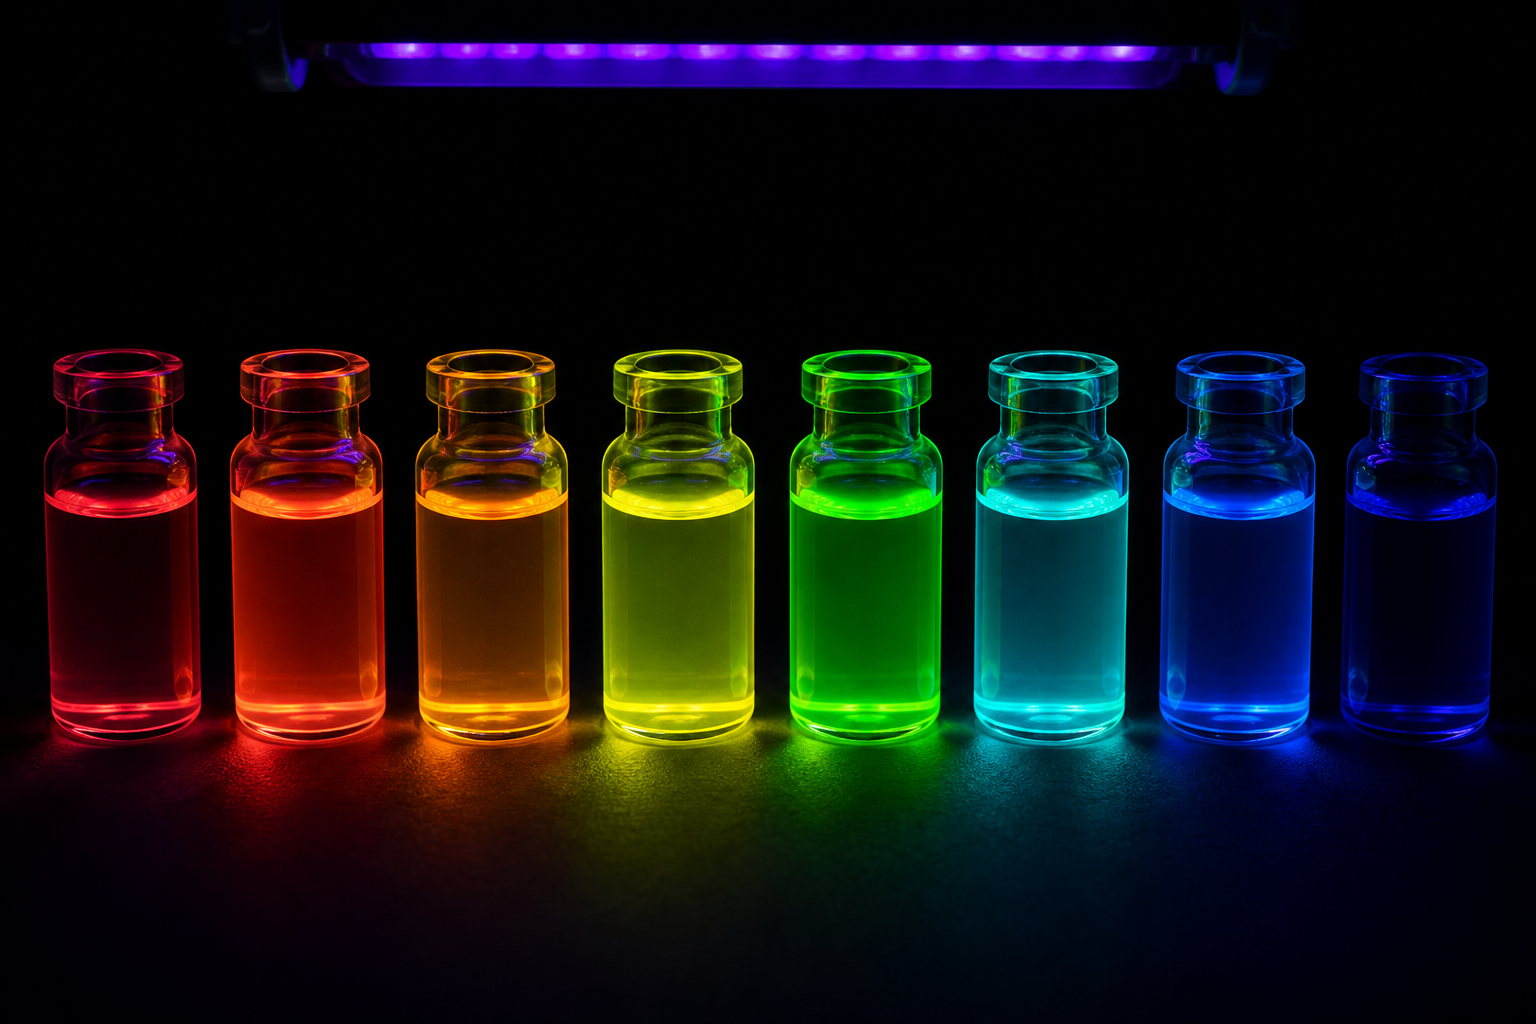
\includegraphics[width=0.58\linewidth]{images/book5/ai/b5-07-quantum-dot-vials.png}

{\small Puntos cuánticos bajo luz ultravioleta: el mismo semiconductor, en cristales cada vez más pequeños, brilla del rojo al azul. El color lo fijan las energías de partícula en una caja de este capítulo --- confinamiento que se ve.}
\end{omfigure}

\section{Ejercicios}

\begin{exercise}[$\star$]\label{exo:b3:schrodinger-three-dimensions:1}
El estado gaussiano $\psi(\vect r) = A\,\eu^{-r^2/4\sigma^2}$. (a)
Normalícese ($\int_0^\infty x^2\eu^{-x^2}\dd x = \sqrt\pi/4$). (b)
Calcúlense $\langle r^2\rangle$ y $\Delta x$ (la isotropía ayuda). (c)
¿Cuál es $\vect\jmath$ para este estado y por qué? (d) Multiplíquese por
$\eu^{\iu\vect k_0\cdot\vect r}$: ¿cuánto valen ahora $\langle\vect
p\rangle$ y $\vect\jmath$?
\end{exercise}

\begin{exercise}[$\star$]\label{exo:b3:schrodinger-three-dimensions:2}
Para la caja cúbica, enumérense todos los niveles hasta $E = 15$ (en unidades
de $h^2/8ma^2$) con sus degeneraciones. Muéstrese después que el nivel $27$
es degenerado \emph{más allá} de las permutaciones: hállense sus dos familias
de números cuánticos y dígase por qué esa degeneración ``accidental'' no se
sigue de la simetría cúbica.
\end{exercise}

\begin{exercise}[$\star$]\label{exo:b3:schrodinger-three-dimensions:3}
Calcúlese la corriente $\vect\jmath$ para: (a) la onda plana
$A\eu^{\iu kx}$; (b) la onda estacionaria $A\sin kx$; (c) la
superposición $A(\eu^{\iu kx} + r\,\eu^{-\iu kx})$, con $r$ real ---
interprétese el resultado como el flujo incidente menos el reflejado; (d) el
estado $A\,\eu^{\iu m\varphi}$ sobre un anillo de radio $b$ (úsese allí $|\vect\nabla|
= (1/b)\partial_\varphi$): una corriente que circula eternamente.
\end{exercise}

\begin{exercise}[$\star$]\label{exo:b3:schrodinger-three-dimensions:4}
Un cristalito de punto cuántico confina un par electrón--hueco de masa
efectiva $\mu = 0.10\,m_{\text{e}}$; la energía del fotón que emite es la
banda prohibida del material masivo $E_{\text{g}} = \qty{1.74}{eV}$ más la
energía de confinamiento de una caja esférica, $\pi^2\hbar^2/2\mu R^2$. (a)
Calcúlese la energía de confinamiento en $R = \qty{3}{nm}$. (b) La longitud de
onda emitida. (c) ¿Hacia dónde se desplaza el color al encoger el punto? (d)
¿Por qué muestra un solo color fijo el seleniuro de cadmio masivo ($R$
grande)?
\end{exercise}

\begin{exercise}[$\star\star$]\label{exo:b3:schrodinger-three-dimensions:5}
Una partícula en un anillo (radio $b$, coordenada $\varphi$): los estados
estacionarios son $\psi_m = \eu^{\iu m\varphi}/\sqrt{2\pi}$. (a)
¿Por qué debe ser $m$ entero? (b) Muéstrese que $E_m = \hbar^2m^2/2mb^2$ ---
cuidado con las dos $m$: escríbase $E_m = \hbar^2 m^2/2Mb^2$ para una masa
$M$ --- y obsérvese que cada nivel con $m \neq 0$ es doblemente degenerado:
¿qué simetría empareja $+m$ con $-m$? (c) Calcúlense la corriente de
$\psi_m$ y el momento magnético ``orbital'' asociado si la partícula lleva
la carga $q$. (d) Los seis electrones móviles del benceno viven sobre un
anillo de $b \approx \qty{1.4}{\angstrom}$: estímese la energía del fotón de
la primera excitación permitida ($m = \pm1 \to \pm2$) y compárese con la
absorción ultravioleta del benceno cerca de \qty{180}{nm} --- un anillo, sin
química alguna.
\end{exercise}

\begin{exercise}[$\star\star$]\label{exo:b3:schrodinger-three-dimensions:6}
Degeneraciones del oscilador isótropo. (a) Muéstrese que el número de
ternas con $n_x + n_y + n_z = n$ es $(n+1)(n+2)/2$. (b) Enumérense las
poblaciones de capa para $n = 0$ hasta $3$, duplicadas por el espín. (c)
Muéstrese que los llenados acumulados son $2, 8, 20, 40, \dots$: los tres
primeros coinciden con los números ``mágicos'' de nucleones especialmente
estables de la física nuclear --- ¿qué sugiere el fallo en $40$ (los mágicos
reales son $28$ y $50$) sobre el potencial nuclear? (d) ¿Por qué el patrón
irregular de niveles de la caja, a diferencia del del oscilador, no produce
una estructura de capas marcada?
\end{exercise}

\begin{exercise}[$\star\star$]\label{exo:b3:schrodinger-three-dimensions:7}
El pozo esférico infinito (radio $R$): usando el truco de la onda $s$,
(a) hállense los niveles $E_n = n^2\pi^2\hbar^2/2MR^2$ y las funciones de onda
$u_n$; (b) calcúlese $E_1$ para un nucleón ($Mc^2 =
\qty{939}{MeV}$) en $R = \qty{5}{fm}$ (úsese $\hbar c =
\qty{197.3}{MeV.fm}$); (c) compárese con los espaciados de niveles de
nucleón medidos, de unos pocos MeV en núcleos medianos; (d) ¿dónde es más
probable hallar la partícula en el estado fundamental? Calcúlese el máximo de
$|u_1|^2$ y contrástelo con la respuesta de la caja unidimensional para
$|\varphi|^2$.
\end{exercise}

\begin{exercise}[$\star\star$]\label{exo:b3:schrodinger-three-dimensions:8}
Contar electrones en un metal. (a) A partir de la
\cref{prop:b3:schrodinger-three-dimensions:counting} con dos estados de
espín, muéstrese que llenar con $N$ electrones un volumen $V$ alcanza la
energía de Fermi
\[
E_{\text{F}} = \frac{\hbar^2}{2m_{\text{e}}}\,(3\pi^2n)^{2/3} ,
\qquad n = N/V .
\]
(b) Evalúese para el cobre. (c) Calcúlense la velocidad de Fermi
correspondiente y la temperatura $E_{\text{F}}/k_{\text{B}}$. (d) En una
frase: ¿por qué no se sitúan todos los electrones en el estado fundamental y
qué principio (anticipado aquí y demostrado en el
\cref{ch:b3:identical-particles}) lo prohíbe?
\end{exercise}

\begin{exercise}[$\star\star$]\label{exo:b3:schrodinger-three-dimensions:9}
Profundidad mínima de un pozo esférico. Para el pozo finito ($-V_0$ para
$r < R$), el estado fundamental de onda $s$ tiene $u = \sin kr$ dentro y
$\eu^{-\kappa r}$ fuera. (a) Escríbanse $k$ y $\kappa$ y la
condición de empalme $k\cot kR = -\kappa$. (b) Muéstrese que un estado
ligado aparece por primera vez cuando $kR = \pi/2$, exactamente en $E = 0$,
lo que da $V_{0,\min} = \pi^2\hbar^2/8MR^2$. (c) Evalúese para el deuterón
($M \to \mu = m_{\text{p}}/2$, $R = \qty{2.1}{fm}$). (d) Contrástelo
con una dimensión, donde liga incluso el pozo más somero: ¿qué cambia
físicamente la pared $u(0) = 0$?
\end{exercise}

\begin{exercise}[$\star\star\star$]\label{exo:b3:schrodinger-three-dimensions:10}
El deuterón, resuelto. Con $\mu c^2 = \qty{469}{MeV}$, $R =
\qty{2.1}{fm}$, $B = \qty{2.22}{MeV}$: (a) calcúlese $\kappa$ a partir de $B$
y la longitud de la cola $1/\kappa$; (b) escríbase la condición de empalme y
muéstrese que se convierte en $\cot kR = -\kappa/k$ con $k$ fijado por
$V_0 - B$; (c) resuélvase para $V_0$ (itérese: pártase de $kR \approx 0.6\pi$) y
dese $V_0$ al MeV más próximo; (d) calcúlese la probabilidad de que los
nucleones estén separados más de $R$ (intégrese la cola) y coméntese lo de ``un
núcleo que vive sobre todo fuera de su propia fuerza''.
\end{exercise}

\begin{exercise}[$\star\star\star$]\label{exo:b3:schrodinger-three-dimensions:11}
Ehrenfest y la continuidad en tres dimensiones. (a) Muéstrese
$\dd\langle\vect r\rangle/\dd t = \langle\vect p\rangle/m$ a partir de la
ecuación de continuidad (intégrese $\vect r\,\partial_t\rho$ por partes).
(b) Muéstrese $\dd\langle\vect p\rangle/\dd t =
-\langle\vect\nabla V\rangle$. (c) ¿Bajo qué condición sobre $V$ sigue
$\langle\vect r\rangle$ exactamente la trayectoria clásica? (d)
Dese un caso concreto en el que no lo hágase (un paquete separado por un
potencial de doble rendija, por ejemplo) y explíquese qué describe entonces el
promedio.
\end{exercise}

\begin{exercise}[$\star\star\star$]\label{exo:b3:schrodinger-three-dimensions:12}
Por qué no colapsan los átomos. Modelícese el estado fundamental del
hidrógeno con la función de prueba $\psi \propto \eu^{-r/a}$, con $a$
ajustable. (a) Admitiendo $\langle E_k\rangle = \hbar^2/2m_{\text{e}}a^2$ y
$\langle E_p\rangle = -e^2/4\pi\varepsilon_0a$, explíquese el origen de cada
dependencia. (b) Minimícese $E(a)$ y muéstrese que el óptimo es el radio de
Bohr, con $E = \qty{-13.6}{eV}$. (c) ¿Por qué \emph{eleva} la energía
encoger $a$ por debajo del óptimo, aunque el potencial se ahonde? (d) El
mismo argumento con el $1/r$ sustituido por la atracción gravitatoria entre
electrón y protón: hállese el ``radio de Bohr gravitatorio'' y conclúyase por
qué la gravedad no construye átomos.
\end{exercise}

\section{Problema: el color de un punto cuántico}

\begin{problem}[{Problema de fin de semana --- fabricar luz contando
nanómetros}]\label{pb:b3:schrodinger-three-dimensions:1}
El Premio Nobel de Química de 2023 recayó en el descubrimiento y la síntesis
de los puntos cuánticos: cristalitos tan pequeños que las energías de
partícula en una caja de este capítulo fijan su color, y que hoy brillan en
las pantallas de televisión y marcan moléculas en células vivas. Este
problema diseña una pantalla de puntos a partir de la ecuación de
Schrödinger. Modelo: el par electrón--hueco ópticamente activo, de masa
efectiva $\mu = 0.10\,m_{\text{e}}$
($m_{\text{e}}c^2 = \qty{511}{keV}$), confinado en una esfera de radio
$R$; energía del fotón emitido
\[
E(R) = E_{\text{g}} + \frac{\pi^2\hbar^2}{2\mu R^2} ,
\]
con la banda prohibida del material masivo $E_{\text{g}} = \qty{1.74}{eV}$
(seleniuro de cadmio). Úsense $\hbar c = \qty{197.3}{eV.nm}$ y $hc =
\qty{1240}{eV.nm}$.

\medskip\noindent\textbf{Parte I --- La física de la fórmula.}
\begin{enumerate}
  \item ¿De dónde sale el término $\pi^2\hbar^2/2\mu R^2$? Dedúzcase como
        el nivel fundamental del pozo esférico infinito mediante la
        sustitución de onda $s$.
  \item ¿Por qué \emph{eleva} siempre el confinamiento la energía emitida y
        nunca la baja?
  \item Evalúese la energía de confinamiento para $R = 10$, $4$, $2$ y
        \qty{1}{nm}, e identifíquese el tamaño a partir del cual deja de ser
        una corrección pequeña a $E_{\text{g}}$.
  \item El modelo ignora la atracción electrón--hueco. ¿En qué sentido
        desplazaría la emisión incluirla, y por qué es mejor la
        aproximación para los puntos \emph{pequeños} (compárense las
        dependencias $1/R^2$ y $1/R$)?
  \item ¿A qué longitud de onda emite el seleniuro de cadmio masivo? ¿En
        qué parte del espectro cae?
  \item ¿Por qué brilla un vaso de disolución de puntos en \emph{un} solo
        color puro, aunque contenga $10^{15}$ puntos? ¿Qué propiedad de la
        síntesis queda así certificada?
\end{enumerate}

\medskip\noindent\textbf{Parte II --- Diseñar la paleta.}
Una pantalla necesita rojo a \qty{630}{nm}, verde a \qty{530}{nm} y azul a
\qty{460}{nm}.
\begin{enumerate}[resume]
  \item Conviértase cada longitud de onda en una energía de fotón.
  \item Para cada color, calcúlense la energía de confinamiento necesaria y
        el radio del punto.
  \item Hágase una tabla: ¿cuántos átomos de anchura tiene cada punto,
        aproximadamente (espaciado reticular $\approx \qty{0.6}{nm}$)?
  \item El azul es el más difícil para los puntos de seleniuro de cadmio:
        explíquese por qué a partir de sus radios (¿qué le ocurre a la
        tolerancia cuando $R$ se reduce?).
  \item Muéstrese que la sensibilidad de la energía emitida al tamaño es
        \[
        \frac{\dd E}{\dd R} = -\frac{\pi^2\hbar^2}{\mu R^3} ,
        \]
        y evalúese, en $\unit{meV}$ por nanómetro, en el radio del punto
        verde.
  \item Un lote varía un $\pm5\%$ en radio: calcúlese la dispersión de
        longitud de onda de la emisión verde y compárese con la anchura de
        línea de $\sim\qty{25}{nm}$ que tolera una buena pantalla.
  \item ¿Por qué tuvieron que esperar las pantallas de puntos cuánticos a
        una química capaz de controlar el tamaño a \emph{escala atómica}, y
        por qué es eso un logro de nivel Nobel?
\end{enumerate}

\medskip\noindent\textbf{Parte III --- Más brillantes, más puros, más extraños.}
\begin{enumerate}[resume]
  \item Los televisores modernos usan los puntos como convertidores de
        color: un led azul ilumina puntos rojos y verdes. ¿Por qué debe
        superar la energía del fotón de bombeo a la energía de emisión del
        punto, y adónde va la diferencia?
  \item Calcúlese la fracción de la energía de un fotón de bombeo de
        \qty{460}{nm} que se pierde como calor cuando se emite un fotón
        rojo de \qty{630}{nm}.
  \item Un punto puede además \emph{absorber} en muchas longitudes de onda
        y \emph{emitir} en una sola: explíquese, a partir de la estructura de
        niveles, por qué la absorción es de banda ancha y la emisión,
        estrecha.
  \item Los biólogos marcan proteínas con puntos de varios tamaños
        excitados por una sola lámpara ultravioleta: ¿qué propiedad de los
        puntos hace bastar una lámpara donde los colorantes orgánicos
        necesitan un láser por color?
  \item Estímese el número de átomos del punto rojo ($4/3\pi R^3$, con un
        volumen atómico $\sim(\qty{0.3}{nm})^3$): ¿es ``átomo artificial''
        un nombre justo para un objeto de este tamaño con niveles
        discretos?
  \item En una frase: ¿qué desempeña el papel del ``núcleo'' en este átomo
        artificial, es decir, qué retiene al electrón?
\end{enumerate}

\medskip\noindent\textbf{Parte IV --- El confinamiento por toda la física.}
\begin{enumerate}[resume]
  \item La misma estimación $E_1 \sim \pi^2\hbar^2/2MR^2$ aplicada a un
        nucleón en $R = \qty{3}{fm}$ da ¿qué escala de energía? (Es la
        razón por la que la física nuclear habla en MeV).
  \item Aplicada a un electrón confinado a tamaño nuclear, da ¿qué energía
        escandalosa? ¿Y qué argumenta eso sobre los electrones ``dentro''
        del núcleo (un argumento que en su día mató una teoría de la
        desintegración beta)?
  \item Aplicada a una persona de \qty{70}{kg} en una habitación de \qty{2}{m}:
        calcúlese la energía de confinamiento y conclúyase.
  \item Inviértase la fórmula: ¿a qué tamaño de confinamiento alcanza la
        energía de confinamiento de un \emph{electrón} su \omterm{def:b3:relativistic-dynamics:momentum-energy}{energía en reposo}
        $m_{\text{e}}c^2$, y qué física nueva (la creación de pares de
        partículas, \cref{ch:b3:relativistic-dynamics}) advierte de que la
        ecuación de Schrödinger de una partícula está entonces fuera de su
        alcance?
  \item Enúnciese la ley de escala general: energía de confinamiento frente a
        masa y frente a tamaño.
  \item Resúmase el resultado con nombre propio: una sola fórmula,
        $E_{\text{g}} + \pi^2\hbar^2/2\mu R^2$, convierte radios de
        $4.0$, $2.5$ y \qty{2.0}{nm} en rojo, verde y azul --- color
        fabricado contando nanómetros y a la venta en cualquier tienda de
        electrónica.
\end{enumerate}
\end{problem}
